\documentclass[english, 11 pt, class=article, crop=false]{standalone}
%\documentclass[english, 11 pt]{report}
\usepackage[T1]{fontenc}
\usepackage[utf8]{luainputenc}
\usepackage{babel}
\usepackage[hidelinks, bookmarks]{hyperref}
\usepackage{geometry}
\geometry{verbose,tmargin=1cm,bmargin=3cm,lmargin=4cm,rmargin=4cm,headheight=3cm,headsep=1cm,footskip=1cm}
\setlength{\parindent}{0bp}
\usepackage{amsmath}
\usepackage{amssymb}
\usepackage{esint}
\usepackage{import}
\usepackage[subpreambles=false]{standalone}
%\makeatletter
\addto\captionsenglish{\renewcommand{\chaptername}{Kapittel}}
\makeatother
\usepackage{tocloft}
\addto\captionsenglish{\renewcommand{\contentsname}{Innhold}}
\usepackage{graphicx}
\usepackage{placeins}
\raggedbottom
\usepackage{calc}
\usepackage{cancel}
\makeatletter
\usepackage{color}
\definecolor{shadecolor}{rgb}{0.105469, 0.613281, 1}
\usepackage{framed}
\usepackage{wrapfig}
\usepackage{bm}
\usepackage{ntheorem}

\usepackage{ragged2e}
\RaggedRight
\raggedbottom
\frenchspacing

\newcounter{lign}[section]
\newenvironment{lign}[1][]{\Large \refstepcounter{lign} \large
	\textbf{\thelign #1} \rmfamily}{\par\medskip}
\numberwithin{lign}{section}
\numberwithin{equation}{section}
\usepackage{xcolor}
\usepackage{icomma}
\usepackage{mathtools}
\usepackage{lmodern} % load a font with all the characters
\usepackage{xr-hyper}
\makeatother
\usepackage[many]{tcolorbox}

%\setlength{\parskip}{\medskipamount}
\newcommand{\parskiplength}{11pt}
%\setlength{\parskip}{0 pt}
\newcommand\eks[2][]{\begin{tcolorbox}[enhanced jigsaw,boxrule=0.3 mm, arc=0mm,breakable,colback=green!30] {\large \textbf{Eksempel #1} \vspace{\parskiplength}\\} #2 \vspace{1pt} \end{tcolorbox}\vspace{1pt}}

\newcommand\fref[2][]{\hyperref[#2]{\textsl{Figur \ref*{#2}#1}}}
\newcommand{\hr}[2]{\hyperref[#2]{\color{blue}\textsl{#1}}}

\newcommand\rgg[2][]{\begin{tcolorbox}[boxrule=0.3 mm, arc=0mm,colback=orange!55] #2 \vspace{1pt} \end{tcolorbox}\vspace{-2pt}}
\newcommand\alg[1]{\begin{align*} #1 \end{align*}}
\newcommand\algv[1]{\vspace{-11 pt} \begin{align*} #1 \end{align*}}
\newcommand\vs{\vspace{-11 pt}}
\newcommand\g[1]{\begin{center} {\tt #1}  \end{center}}
\newcommand\gv[1]{\begin{center} \vspace{-22 pt} {\tt #1} \vspace{-11 pt} \end{center}}
%\addto\captionsenglish{\renewcommand{\contentsname}{Løsningsforslag tentamen R2 H2015}}

% Farger
\colorlet{shadecolor}{blue!30} 

% Figur
\usepackage{float}
\usepackage{subfig}
\captionsetup[subfigure]{labelformat=empty}
\usepackage{esvect}

\newcommand\sv{\textbf{Svar:} \vspace{5 pt} \\}

%Tableofconents
\renewcommand{\cfttoctitlefont}{\Large\bfseries}
\setlength{\cftsubsecindent}{2 cm}
\newcommand\tocskip{6 pt}
\setlength{\cftaftertoctitleskip}{30 pt}
\setlength{\cftbeforesecskip}{\tocskip}
%\setlength{\cftbeforesubsecskip}{\tocskip}

%Footnote:
\usepackage[bottom, hang, flushmargin]{footmisc}
\usepackage{perpage} 
\MakePerPage{footnote}
\addtolength{\footnotesep}{2mm}
\renewcommand{\thefootnote}{\arabic{footnote}}
\renewcommand\footnoterule{\rule{\linewidth}{0.4pt}}

%asin, atan, acos
\DeclareMathOperator{\atan}{atan}
\DeclareMathOperator{\acos}{acos}
\DeclareMathOperator{\asin}{asin}

%Tabell
\addto\captionsenglish{\renewcommand{\tablename}{Figur}}

% Figur
\usepackage[font=footnotesize,labelfont=sl]{caption}
\addto\captionsenglish{\renewcommand{\figurename}{Figur}}

% Figurer
\newcommand\scr[1]{/home/sindre/R/scr/#1}
\newcommand\asym[1]{/home/sindre/R/asymptote/#1}

%Toc for seksjoner
\newcommand\tsec[1]{\phantomsection\addcontentsline{toc}{section}{#1}
	\section*{#1}}
%\newcommand\tssec[1]{\subsection*{#1}\addcontentsline{toc}{subsection}{#1}}
\newcommand\tssec[1]{\subsection*{#1}}
% GeoGebra
\newcommand{\cms}[2]{{\tt #1( #2 )}}
\newcommand{\cm}[2]{{\large \tt #1( #2 )} \gvs \\}
\newcommand{\cmc}[2]{{\large \tt #1( #2 )} \large (CAS)  \gvs \\ \normalsize}
\newcommand{\cmk}[2]{{\large \tt #1( #2 )} \large (Inntastingsfelt)  \gvs \\ \normalsize}

\newcommand\gvs{\vspace{11 pt}}

\newcommand\vsk{\vspace{11 pt}}
\newcommand{\merk}{\vsk \textsl{Merk}: }
\newcommand{\fig}[1]{
\begin{figure}
	\centering
	\includegraphics[scale=0.5]{fig/#1}
\end{figure}
}
\newcommand{\figc}[1]{
		\centering
		\includegraphics[scale=0.5]{fig/#1}
}

% Opg
%\newcommand{\opgt}{\phantomsection \addcontentsline{toc}{section}{Oppgaver} \section*{Oppgaver for kapittel \thechapter}}
\newcounter{opg}
\numberwithin{opg}{section}

\newcommand{\opl}[1]{\vspace{15pt} \refstepcounter{opg} \textbf{\theopg} \vspace{2 pt} \label{#1} \\}




\begin{document}
\newpage

\subimport{/home/sindre/R/ggb/}{ncmd}
\addtocontents{toc}{\protect\vspace{10pt}}
\setlength{\cftbeforesecskip}{20 pt}
\tsec{Grafikkfeltet}

\tssec{Funksjoner på et gitt intervall}
I mange oppgaver jobber vi med funksjoner som er definert på et gitt intervall. Når vi på eksamen skal levere grafen til en slik funksjon, er det krav om at vi tegner grafen bare på intervallet som er oppgitt.\vsk

La oss bruke funksjonenen
\[ A(x)=x^3+4x^2+x-2\quad,\quad x\in[-4, 1] \]
som eksempel. For å tegne grafen til $ A $ på intervallet $ {-4\leq x \leq 1} $, bruker vi kommandoen \texttt{Funksjon( <Funksjon>, <Start>, <Slutt> )}. Vi skriver da:
\g{A = Funksjon( (x-1)(x+2)(x+3)+4, -4, 1 )}
\begin{figure}[H]
	\centering
	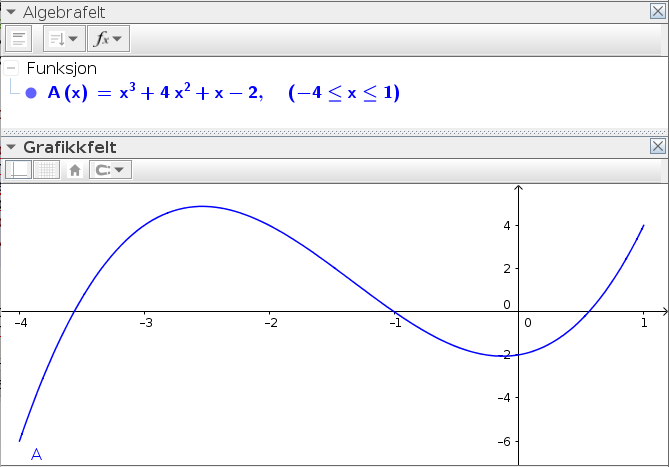
\includegraphics[scale=0.5]{fig/funk}
\end{figure}
\textsl{Husk}: Aksene justeres\footnote{Grafen bør strekke seg så godt over grafikkfeltet som mulig, men aller vikigst er at grafen er synlig på hele intervallet til definisjonsmengden.} ved enten å bruke {\tt Flytt grafikkfelt} \big(\;
\includegraphics[scale=0.25]{fig/flytt}\;\big), eller ved å holde inne {\tt shift}-knappen på tastaturet mens man drar over aksene. 
\tssec{Nullpunkter og ekstremalpunkter gå gitt intervall}
Når vi må definere funksjoner på et bestemt intervall, blir vi stilt ovenfor et lite problem når vi skal finne nullpunter og ekstremalpunkter. I figuren under har vi først definert funksjonen $ f(x)=\sin(\pi x) $, og deretter $ g $ som $ f $ for $x \in[-3, 3] $.\\ ( \texttt{g = Funksjon( f, -3, 3 )} ).
\begin{figure}[H]
	\centering
	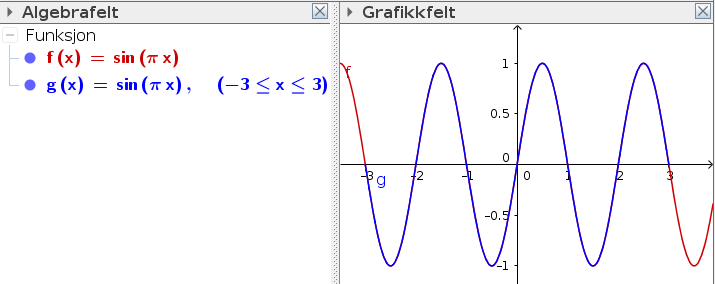
\includegraphics[scale=0.5]{fig/sin0}
\end{figure}
Tenk nå at vi vi GeoGebra ønsker å finne alle nullpunktene til $ g $. For funksjoner som ikke består av polynomuttrykk, må vi bruke kommandoen \cms{NullpunktIntervall}{<Funksjon>, <Start>, <Slutt>}. Vi skriver derfor:
\g{NullpunktIntervall[ g, -3, 3]}
\begin{figure}[H]
	\centering
	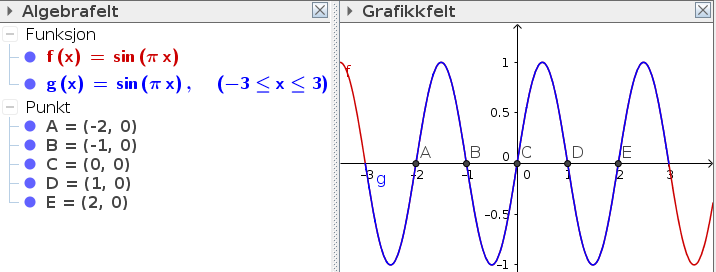
\includegraphics[scale=0.5]{fig/sin}
\end{figure}
Men $ g $ har åpenbart nullpunkt for ${ x\in\lbrace-3, 3\rbrace }$ også, vi mangler altså to nullpunkt! Dette kommer av \texttt{NullpunktIntervall}-kommandoen bare finner \textit{lokale} nullpunkt (se \textsl{vedlegg E} i teoridelen), hvis endepunktene er nullpunkt blir de altså ikke markert.  Fordelen med å først definere\footnote{f er definert for alle $ x\in \mathbb{R} $ og har dermed ingen endepunkt.} $ f $ og deretter $ g $, er at om vi skriver \texttt{NullpunktIntervall[ f, -3, 3]}, får vi det vi ønsker (de gamle punktene \texttt{A}-\texttt{E} er først slettet):
\begin{figure}[H]
	\centering
	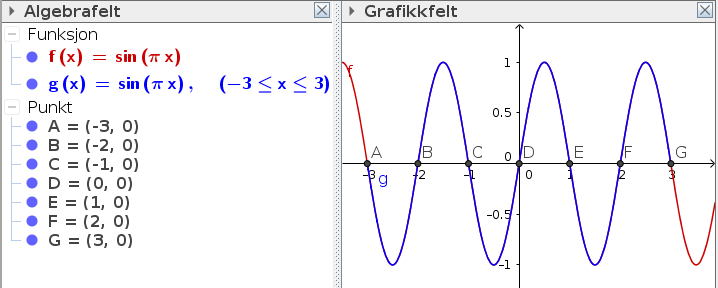
\includegraphics[scale=0.5]{fig/sin2}
\end{figure}

Problemet, og løsningen av det, vil være akkurat de samme når vi skal finne ekstremalpunkter (\cms{Ekstremalpunkt}{<Funksjon>, <Start>, <Slutt>})
\begin{comment}
	\tssec{Visning av objekter og navn på aksene}
	For å ha et oversiktlig grafikkfelt, kan det noen ganger være hendig å fjerne eller legge til visningen av objekter og navn. Hvis man høyreklikker på et objekt i algebrafeltet, kan man huke av for disse to valgene. 
	\fig{valg}
	Det kan også være ønskelig å legge inn egne tekstbokser (spesielt på aksene), dette kan gjøres ved å velge {\tt Tekst} fra verkyøymenyen.
	\fig{tekst}
\end{comment}
\tsec{CAS}
\tssec{Definere variabler \label{defvar}}
Hvis vi ønsker å definere variabler som vi skal bruke i andre celler, må vi skrive \texttt{:=} . I figuren under er forskjellen mellom \texttt{=} og \texttt{:=} demonstrert med et forsøk på å finne $ f'(x) $ til funksjonen $ f(x)=x^2 $:
\begin{figure}
	\centering
	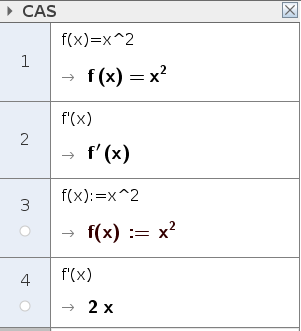
\includegraphics[scale=0.5]{fig/fder}
\end{figure}
Av figuren legger vi også merke til at celle 3 og celle 4 er markert med en hvit runding. Dette indikerer at størrelsen vil vises i \textsl{Grafikkfelt} eller \textsl{Grafikkfelt 3D} hvis man trykker på markøren (den skal da bli blå).
\tssec{Celle-referanser}

Ofte kommer vi ut for situasjoner der vi ønsker å bruke uttrykket vi har funnet i tidligere celler. Som eksempel har vi i celle 1 skrevet inn volumet $ v $ av en kule med radius $ r $, mens i celle 2 har vi volumet $ V $ av en kule med radius $ R $. Ønsker vi å finne forholdet mellom disse, kan vi bruke cellereferanser som hjelpemiddel. For å referere til celle 1 skriver vi \texttt{\$1} og for celle 2 skriver vi \texttt{\$2}. Forholdet $ \frac{v}{V} $ kan vi da skriver som \texttt{\$1/\$2}:
\begin{figure}
	\centering
	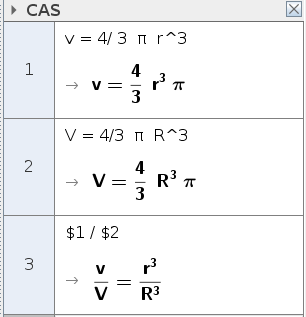
\includegraphics[scale=0.5]{fig/ref}
\end{figure}

\tssec{Lister}
Når et uttrykk står inni sløyfeparanteser \{\}, betyr det at det er laget en liste. En liste inneholder flere elementer som vi kan hente ut. Dette gjør vi ved å skrive paranteser bak listen, hvor vi angir nummeret til elementet i listen.
\begin{figure}
	\centering
	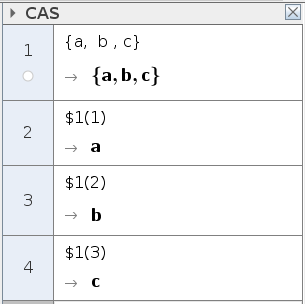
\includegraphics[scale=0.5]{fig/liste}
\end{figure}

Lister bruker vi også når vi skal løse liginger med flere ukjente:
\begin{figure}
	\centering
	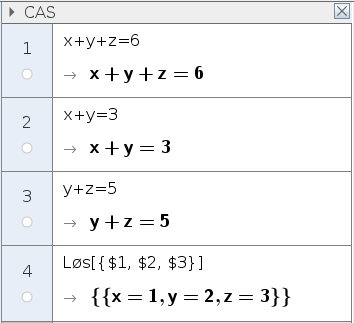
\includegraphics[scale=0.5]{fig/lign}
\end{figure}
\tssec{Høyre- og venstresiden \label{hogl}}
De fleste uttrykkene vi jobber med i CAS inneholder et $ = $ tegn. Disse uttrykkene er en ligning med en venstre- og høyreside. Ofte ønsker vi å bruke uttrykket på bare én av disse sidene, og oftest høyresiden. Som eksempel har vi løst ligningen $ (a+b)x = c $ og definert funksjonen $ f(x)= d x^2 $. Vi ønsker så å sette løsningen av ligningen inn i funksjonen. Dette gjør vi ved hjelp av \texttt{HøyreSide}-kommandoen (resulatet uten bruken av denne er vist i celle 4).
\begin{figure}
	\centering
	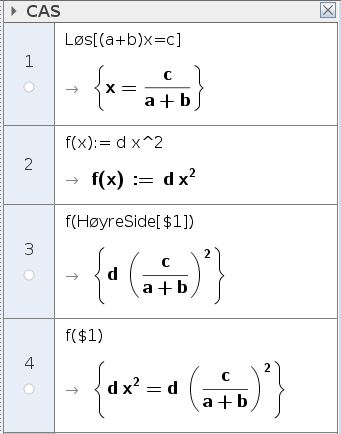
\includegraphics[scale=0.5]{fig/hoyre}
\end{figure}
\tssec{ByttUt}
Noen ganger ønsker vi å endre en variabel i et utrykk. For å gjøre dette kan vi anvende \cms{ByttUt}{<Uttrykk>, <Liste med forandringer>}. La oss se på uttrykket
\[ \frac{a+b}{c} \]
Vi ønsker nå å sette $ {a=d }$, $ {b=2} $ og $ {c=f} $. Dette kan vi gjør ved å skrive følgende:
\begin{figure}
	\centering
	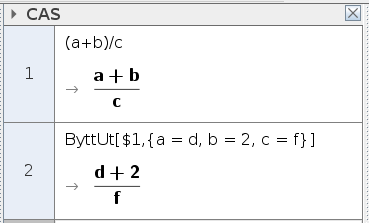
\includegraphics[scale=0.5]{fig/cas2}
\end{figure}

En typisk oppgave i R2 kan være å løse en differensialligning av andre orden med initialbetingelser, og deretter bruke denne løsningen videre i oppgaven. Oppgaven handler ofte om noe som endrer seg med tiden. Når CAS løser differensialligninger, blir resultatet en funksjon $ y(x) $. Vi kan da bruke \texttt{ByttUt}-kommandoen for å definere en ny funksjon $ f(t) $.
\begin{figure}
	\centering
	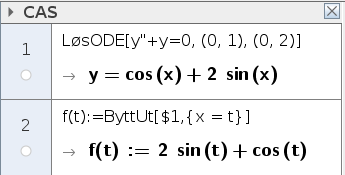
\includegraphics[scale=0.5]{fig/ode}
\end{figure}

\end{document}
